\documentclass[aspectratio=169,12pt]{beamer}

% --- Theme & Colors ---
\usetheme{default}
\usecolortheme{default}
\usefonttheme{professionalfonts}

\definecolor{deepblue}{RGB}{15,40,90}
\definecolor{accentblue}{RGB}{30,90,200}
\definecolor{accentorange}{RGB}{220,100,20}
\definecolor{lightgray}{RGB}{245,245,248}
\definecolor{midgray}{RGB}{120,120,130}
\definecolor{textgray}{RGB}{50,50,60}
\definecolor{greenok}{RGB}{30,130,60}
\definecolor{redbad}{RGB}{180,30,30}

\setbeamercolor{background canvas}{bg=white}
\setbeamercolor{frametitle}{fg=deepblue,bg=white}
\setbeamercolor{normal text}{fg=textgray}
\setbeamercolor{itemize item}{fg=accentblue}
\setbeamercolor{itemize subitem}{fg=midgray}

\setbeamertemplate{navigation symbols}{}
\setbeamertemplate{footline}{%
  \hbox{%
    \begin{beamercolorbox}[wd=.7\paperwidth,ht=2.5ex,dp=1.5ex,leftskip=0.5em]{normal text}%
      \scriptsize\color{midgray}Composition Determines Diversity \textbullet{} GECCO 2026
    \end{beamercolorbox}%
    \begin{beamercolorbox}[wd=.3\paperwidth,ht=2.5ex,dp=1.5ex,rightskip=0.5em,right]{normal text}%
      \scriptsize\color{midgray}\insertframenumber/\inserttotalframenumber
    \end{beamercolorbox}}%
}
\setbeamertemplate{frametitle}{%
  \vspace{0.35em}
  {\large\bfseries\color{deepblue}\insertframetitle}%
  \vspace{0.15em}
  {\color{accentblue}\hrule height 1.5pt}
  \vspace{0.2em}
}

% --- Packages ---
\usepackage{graphicx}
\usepackage{booktabs}
\usepackage{xcolor}
\usepackage{tikz}
\usetikzlibrary{arrows.meta,positioning,shapes,fit,calc}
\usepackage{amsmath,amssymb}
\usepackage{fontenc}
\usepackage{inputenc}
\usepackage{microtype}
\usepackage{array}
\usepackage{colortbl}
\usepackage{listings}
\lstset{
  basicstyle=\ttfamily\footnotesize,
  breaklines=true,
  keywordstyle=\color{deepblue}\bfseries,
  commentstyle=\color{midgray},
  stringstyle=\color{greenok},
  backgroundcolor=\color{lightgray},
  frame=none,
  xleftmargin=0pt,
  aboveskip=0pt,
  belowskip=0pt,
}

\graphicspath{
  {/home/lyra/projects/categorical-evolution/experiments/video_figures/}
  {/home/lyra/projects/categorical-evolution/experiments/plots/}
}

% --- Slide 1: Title ---
\begin{document}

{
\setbeamertemplate{footline}{}
\begin{frame}[plain]
\vspace{1.5em}
\begin{center}
  {\LARGE\bfseries\color{deepblue} Composition Determines Diversity}\\[0.5em]
  {\large\color{textgray} Categorical Fingerprints of Genetic Algorithms}\\[1.2em]
  {\normalsize Robin Langer \quad Claudius Turing \quad Lyra Vega}\\[0.4em]
  {\small\color{midgray} GECCO 2026 \textbullet{} San Jos\'e, Costa Rica \textbullet{} July 2026}
\end{center}
\vspace{1.5em}
\begin{center}
  \color{accentblue}{\rule{0.5\textwidth}{1.2pt}}
\end{center}
\vspace{1em}
\begin{center}
  {\normalsize\color{textgray}%
    \textit{``How you wire your islands matters more than what you evolve.''}%
  }
\end{center}
\end{frame}
}

% --- Slide 2: The Surprising Claim [AHA] ---
\begin{frame}{The Surprising Claim}
\begin{center}
  \includegraphics[width=0.82\textwidth]{multi_domain_topology_ordering.png}
\end{center}
\vspace{0.2em}
\begin{center}
  \footnotesize
  \color{accentorange}\textbf{Kendall's W = 1.0} \quad
  \color{redbad}\textbf{p = 0.00008} \quad
  \color{deepblue}\textbf{Topology explains 23.9$\times$ more variance than domain}
\end{center}
\end{frame}

% --- Slide 3: Why Should You Care? ---
\begin{frame}{Why Should You Care?}
\begin{columns}[T]
  \begin{column}{0.45\textwidth}
    \textbf{\color{midgray}What practitioners tune}
    \vspace{0.5em}
    \begin{itemize}\setlength\itemsep{0.4em}
      \item[\color{midgray}$\circ$] {\color{midgray}Operator selection}
      \item[\color{midgray}$\circ$] {\color{midgray}Crossover type}
      \item[\color{midgray}$\circ$] {\color{midgray}Mutation rate}
      \item[\color{midgray}$\circ$] {\color{midgray}Population size}
    \end{itemize}
  \end{column}
  \begin{column}{0.45\textwidth}
    \textbf{\color{accentblue}What actually determines diversity}
    \vspace{0.5em}
    \begin{itemize}\setlength\itemsep{0.4em}
      \item[\color{accentblue}$\blacktriangleright$] \textbf{Composition structure}
      \item[\color{accentblue}$\blacktriangleright$] \textbf{Migration topology}
    \end{itemize}
  \end{column}
\end{columns}
\vspace{1.2em}
\begin{center}
  \colorbox{lightgray}{\parbox{0.88\textwidth}{\centering
    \small\color{textgray}
    \textbf{Three recommendations:} (1) Prefer ring/mesh over star.\quad
    (2) Monitor $\lambda_2$, not diversity.\quad
    (3) Close cycles, don't just raise migration rate.
  }}
\end{center}
\end{frame}

% --- Slide 4: Hidden Composition ---
\begin{frame}{The Problem: Hidden Composition}
\begin{columns}[T]
  \begin{column}{0.52\textwidth}
    \vspace{0.3em}
    \colorbox{lightgray}{\parbox{0.94\textwidth}{%
    \ttfamily\footnotesize\color{textgray}%
    \textcolor{redbad}{// selection}\\
    let idx = tournament\_select(\\
    \hspace{1em}\&pop, \&cfg, rng);\\[0.3em]
    \textcolor{redbad}{// crossover}\\
    let child = one\_point\_crossover(\\
    \hspace{1em}\&pop[idx], \&mate, rng);\\[0.3em]
    \textcolor{redbad}{// mutation}\\
    let mutant = point\_mutate(\\
    \hspace{1em}\&child, \&cfg, rng);\\[0.3em]
    \textcolor{redbad}{// evaluate}\\
    let fit = evaluate(\&mutant, \&env);\\
    pop[i] = (mutant, fit);
    }}
  \end{column}
  \begin{column}{0.44\textwidth}
    \vspace{1em}
    \begin{itemize}\setlength\itemsep{0.7em}
      \item Pipeline exists only as \textbf{statement order}
      \item Selection returns an \textbf{index}, not an individual
      \item Randomness \& config \textbf{explicitly threaded}
      \item Composition has \textbf{no formal representation}
    \end{itemize}
    \vspace{0.8em}
    \begin{center}
      \colorbox{lightgray}{\parbox{0.88\textwidth}{\centering
        \small\color{redbad}\textit{You can't ask: does this composition preserve properties of its parts?}
      }}
    \end{center}
  \end{column}
\end{columns}
\end{frame}

% --- Slide 5: Making Composition Explicit [AHA] ---
\begin{frame}{Making Composition Explicit}
\begin{columns}[T]
  \begin{column}{0.48\textwidth}
    \colorbox{lightgray}{\parbox{0.94\textwidth}{%
    \ttfamily\scriptsize\color{midgray}%
    let idx = tournament\_select(\\
    \hspace{1em}\&pop, \&cfg, rng);\\
    let child = one\_point\_crossover(\\
    \hspace{1em}\&pop[idx], \&mate, rng);\\
    let mutant = point\_mutate(\\
    \hspace{1em}\&child, \&cfg, rng);\\
    let fit = evaluate(\&mutant, \&env);\\
    pop[i] = (mutant, fit);\\
    \ldots{} \textcolor{midgray}{(15+ lines)}
    }}
  \end{column}
  \begin{column}{0.48\textwidth}
    \vspace{0.6em}
    \colorbox{white!90!accentblue}{\parbox{0.94\textwidth}{%
    \ttfamily\small\color{deepblue}%
    generationStep fitFunc\\
    \hspace{2em}mutFunc gen =\\
    \hspace{1em}evaluate fitFunc\\
    \hspace{2em}>>>: logGeneration gen\\
    \hspace{2em}>>>: elitistSelect\\
    \hspace{2em}>>>: onePointCrossover\\
    \hspace{2em}>>>: pointMutate mutFunc
    }}
    \vspace{0.5em}
    \begin{center}
      \Large\bfseries\color{accentorange}6 lines. Same algorithm.
    \end{center}
  \end{column}
\end{columns}
\vspace{0.5em}
\begin{center}
  \colorbox{lightgray}{\parbox{0.88\textwidth}{\centering
    \small\color{deepblue}
    \texttt{>>>:} is Kleisli composition --- threads randomness, config, and logging automatically.
    \textbf{The composition is now a first-class value you can type-check, compose, and reason about.}
  }}
\end{center}
\end{frame}

% --- Slide 6: Three Composition Levels ---
\begin{frame}{Three Composition Levels}
\begin{center}
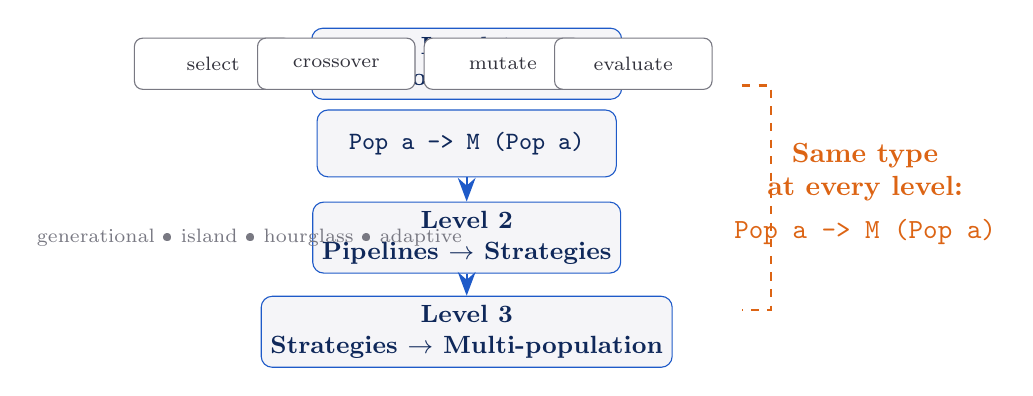
\begin{tikzpicture}[scale=0.92,
  box/.style={draw=accentblue,fill=lightgray,rounded corners=4pt,
              minimum width=3.8cm,minimum height=0.85cm,
              font=\small\bfseries,text=deepblue,align=center},
  op/.style={draw=midgray,fill=white,rounded corners=3pt,
             minimum width=2cm,minimum height=0.65cm,
             font=\scriptsize,text=textgray,align=center},
  arr/.style={-{Stealth[length=3mm]},color=accentblue,thick}
]
  % Level 1
  \node[box] (l1) at (0,0) {Level 1\\Operators $\to$ Pipelines};
  \node[op] (sel) at (-3.5,0) {select};
  \node[op] (cx)  at (-1.8,0) {crossover};
  \node[op] (mut) at (0.5, 0) {mutate};
  \node[op] (ev)  at (2.3, 0) {evaluate};
  % arrows through ops (separate row)
  \node[box] (l1b) at (0,-1.1) {\texttt{Pop a -> M (Pop a)}};
  % Level 2
  \node[box] (l2) at (0,-2.4) {Level 2\\Pipelines $\to$ Strategies};
  \node[font=\scriptsize,text=midgray] at (-3,-2.4) {generational \textbullet{} island \textbullet{} hourglass \textbullet{} adaptive};
  % Level 3
  \node[box] (l3) at (0,-3.7) {Level 3\\Strategies $\to$ Multi-population};
  % Arrows
  \draw[arr] (l1b) -- (l2);
  \draw[arr] (l2)  -- (l3);
  % Same-type annotation
  \node[text=accentorange,font=\normalsize\bfseries,align=center] at (5.5,-1.8)
    {Same type\\at every level:\\[0.3em]\texttt{Pop a -> M (Pop a)}};
  \draw[dashed,color=accentorange,thick] (3.8,-0.3) -- (4.2,-0.3) -- (4.2,-3.4) -- (3.8,-3.4);
\end{tikzpicture}
\end{center}
\begin{center}
  \small\color{midgray}\textit{The composite at every level has the same type as its parts --- a design algebra, not just notation.}
\end{center}
\end{frame}

% --- Slide 7: Domain Invariance ---
\begin{frame}{Domain Invariance}
\begin{columns}[T]
  \begin{column}{0.44\textwidth}
    \vspace{0.4em}
    \begin{tabular}{p{2.8cm}|p{2.8cm}}
      \rowcolor{lightgray}
      \textbf{\color{redbad}Changes} & \textbf{\color{greenok}Invariant} \\
      \midrule
      Genome type & Pipeline shape \\
      Fitness function & Monad stack \\
      Mutation operator & Composition operator \\
       & Strategy combinators \\
    \end{tabular}
    \vspace{1em}
    \small\color{midgray}\textit{Category theory predicts: structure lives in the arrows, not the objects.}
  \end{column}
  \begin{column}{0.52\textwidth}
    \vspace{0.3em}
    \begin{center}
    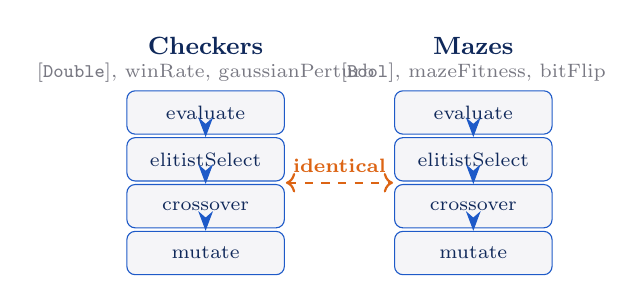
\begin{tikzpicture}[scale=0.85,
      pipe/.style={draw=accentblue,fill=lightgray,rounded corners=3pt,
                   minimum width=2cm,minimum height=0.55cm,
                   font=\scriptsize,text=deepblue,align=center},
      arr/.style={-{Stealth[length=2.5mm]},color=accentblue}
    ]
      % Checkers pipeline
      \node[font=\small\bfseries,text=deepblue] at (0,2.2) {Checkers};
      \node[font=\scriptsize,text=midgray]      at (0,1.8) {[\texttt{Double}], winRate, gaussianPerturb};
      \node[pipe] (ce) at (0,1.2) {evaluate};
      \node[pipe] (cs) at (0,0.5) {elitistSelect};
      \node[pipe] (cc) at (0,-0.2) {crossover};
      \node[pipe] (cm) at (0,-0.9) {mutate};
      \draw[arr] (ce) -- (cs); \draw[arr] (cs) -- (cc); \draw[arr] (cc) -- (cm);
      % Maze pipeline
      \node[font=\small\bfseries,text=deepblue] at (4,2.2) {Mazes};
      \node[font=\scriptsize,text=midgray]      at (4,1.8) {[\texttt{Bool}], mazeFitness, bitFlip};
      \node[pipe] (me) at (4,1.2) {evaluate};
      \node[pipe] (ms) at (4,0.5) {elitistSelect};
      \node[pipe] (mc) at (4,-0.2) {crossover};
      \node[pipe] (mm) at (4,-0.9) {mutate};
      \draw[arr] (me) -- (ms); \draw[arr] (ms) -- (mc); \draw[arr] (mc) -- (mm);
      % Identical annotation
      \draw[<->,dashed,color=accentorange,thick] (1.2,0.15) -- (2.8,0.15)
        node[midway,above,font=\scriptsize\bfseries,color=accentorange]{identical};
    \end{tikzpicture}
    \end{center}
  \end{column}
\end{columns}
\end{frame}

% --- Slide 8: Six Domains ---
\begin{frame}{Six Domains: Maximally Diverse}
\begin{columns}[T]
\begin{column}{0.5\textwidth}
\begin{itemize}\setlength\itemsep{0.5em}
  \item[\textbf{\color{accentblue}1.}] \textbf{OneMax} --- trivially unimodal, binary
  \item[\textbf{\color{accentblue}2.}] \textbf{Maze} --- multi-objective, binary
  \item[\textbf{\color{accentblue}3.}] \textbf{Graph Coloring} --- constraint satisfaction
\end{itemize}
\end{column}
\begin{column}{0.5\textwidth}
\begin{itemize}\setlength\itemsep{0.5em}
  \item[\textbf{\color{accentorange}4.}] \textbf{Knapsack} --- epistatic interactions
  \item[\textbf{\color{accentorange}5.}] \textbf{No Thanks!} --- co-evolutionary, no fixed landscape
  \item[\textbf{\color{accentorange}6.}] \textbf{Checkers} --- intransitive fitness ($A \succ B \succ C \succ A$)
\end{itemize}
\end{column}
\end{columns}
\vspace{1.2em}
\begin{center}
\colorbox{lightgray}{\parbox{0.85\textwidth}{\centering
  \normalsize\color{deepblue}
  If composition determines diversity across \textbf{all six}, it cannot be an artifact of any particular landscape structure.
}}
\end{center}
\vspace{0.6em}
\begin{center}
\includegraphics[width=0.55\textwidth]{domain_comparison.png}
\end{center}
\end{frame}

% --- Slide 9: Experimental Setup ---
\begin{frame}{Experimental Setup}
\begin{columns}[T]
  \begin{column}{0.48\textwidth}
    \vspace{0.5em}
    \begin{tabular}{ll}
      \toprule
      \textbf{Parameter} & \textbf{Value} \\
      \midrule
      Islands & 5 \\
      Individuals/island & 16 \\
      Generations & 100 \\
      Migration rate & 0.1 every 5 gen \\
      Topologies & 5 \\
      Seeds per cell & 30 \\
      \midrule
      \textbf{Total runs} & \textbf{900} \\
      \bottomrule
    \end{tabular}
  \end{column}
  \begin{column}{0.48\textwidth}
    \vspace{0.5em}
    \textbf{Topologies swept:}\\[0.5em]
    \begin{itemize}\setlength\itemsep{0.4em}
      \item None (isolated)
      \item Ring
      \item Star
      \item Random (Erd\H{o}s-R\'enyi, resampled)
      \item Fully connected
    \end{itemize}
    \vspace{0.8em}
    \textbf{Diversity metric:}\\
    \small Normalized pairwise Hamming (binary) / Euclidean (real-valued)
  \end{column}
\end{columns}
\end{frame}

% --- Slide 10: Five Topologies ---
\begin{frame}{Five Topologies and Algebraic Connectivity}
\begin{center}
\includegraphics[width=0.82\textwidth]{topology_networks_lambda2.png}
\end{center}
\begin{center}
\colorbox{lightgray}{\parbox{0.85\textwidth}{\centering
  \small\color{deepblue}
  \textbf{Key quantity:} $\lambda_2$ (algebraic connectivity) --- second-smallest eigenvalue of the graph Laplacian.\\
  Smaller $\lambda_2$ $\Rightarrow$ slower mixing $\Rightarrow$ higher sustained diversity.
  \quad none: $0$ \quad ring: $1.38$ \quad FC: $5.0$
}}
\end{center}
\end{frame}

% --- Slide 11: Universal Ordering [AHA] ---
\begin{frame}{The Universal Ordering}
\begin{columns}[T]
  \begin{column}{0.62\textwidth}
    \includegraphics[width=\textwidth]{multi_domain_topology_ordering.png}
  \end{column}
  \begin{column}{0.35\textwidth}
    \vspace{0.6em}
    \begin{itemize}\setlength\itemsep{0.6em}
      \item \textbf{6 domains.} 900 runs.
      \item \textbf{Identical ordering} in every domain:\\
        none $>$ ring $>$ star $>$ random $>$ FC
      \item \textbf{Kendall's W = 1.0}\\
        (perfect concordance)
    \end{itemize}
    \vspace{0.8em}
    \colorbox{lightgray}{\parbox{\textwidth}{
      \scriptsize
      \color{redbad}$F_{\text{topo}} = 47.8$\quad $F_{\text{domain}} = 0.13$\\
      \color{midgray}Domain: $p = 0.945$ (noise)\\
      \color{accentorange}Topology $>$ Domain: $24\times$
    }}
  \end{column}
\end{columns}
\end{frame}

% --- Slide 12: Spectral Explanation ---
\begin{frame}{The Spectral Explanation}
\begin{columns}[T]
  \begin{column}{0.55\textwidth}
    \includegraphics[width=\textwidth]{lambda2_vs_diversity.png}
  \end{column}
  \begin{column}{0.42\textwidth}
    \vspace{0.5em}
    \begin{itemize}\setlength\itemsep{0.65em}
      \item Diversity follows $\lambda_2$ \textbf{monotonically}
      \item \textbf{None $\to$ Ring} transition:\\ \Large\color{redbad}$-35\%$ diversity
      \normalsize
      \item Each subsequent step:\\ at most $\sim 9\%$ drop
    \end{itemize}
    \vspace{0.8em}
    \colorbox{lightgray}{\parbox{\textwidth}{
      \small\color{deepblue}
      \textbf{First coupling dominates.}\\
      The symmetry-breaking step from isolation to the weakest connection loses a third of diversity.
    }}
  \end{column}
\end{columns}
\end{frame}

% --- Slide 13: Ring/Star Inversion [AHA] ---
\begin{frame}{Falsifiable Prediction: Ring/Star Inversion}
\begin{columns}[T]
  \begin{column}{0.55\textwidth}
    \includegraphics[width=\textwidth]{ring_star_inversion.png}
  \end{column}
  \begin{column}{0.42\textwidth}
    \vspace{0.3em}
    \begin{tabular}{lcc}
      \toprule
      & \textbf{Ring} & \textbf{Star} \\
      \midrule
      $n=5$: $\lambda_2$ & 1.382 & 1.0 \\
      \small(ring $>$ star) & & \\[0.3em]
      $n=7$: $\lambda_2$ & 0.753 & 1.0 \\
      \small(\textbf{star $>$ ring}) & & \\
      \bottomrule
    \end{tabular}
    \vspace{0.8em}
    \textbf{Prediction:} at $n=7$, ring preserves \textit{more} diversity than star.\\[0.5em]
    \textbf{Confirmed (maze, 30 seeds):}\\
    ring $0.387 \pm 0.028$\\
    star $0.336 \pm 0.053$\\
    \color{greenok}$p = 6.6 \times 10^{-5}$ \checkmark\\[0.5em]
    \small\color{midgray}\textit{Not post-hoc. That's science.}
  \end{column}
\end{columns}
\end{frame}

% --- Slide 14: Scope Condition ---
\begin{frame}{Scope Condition: When It Breaks}
\begin{center}
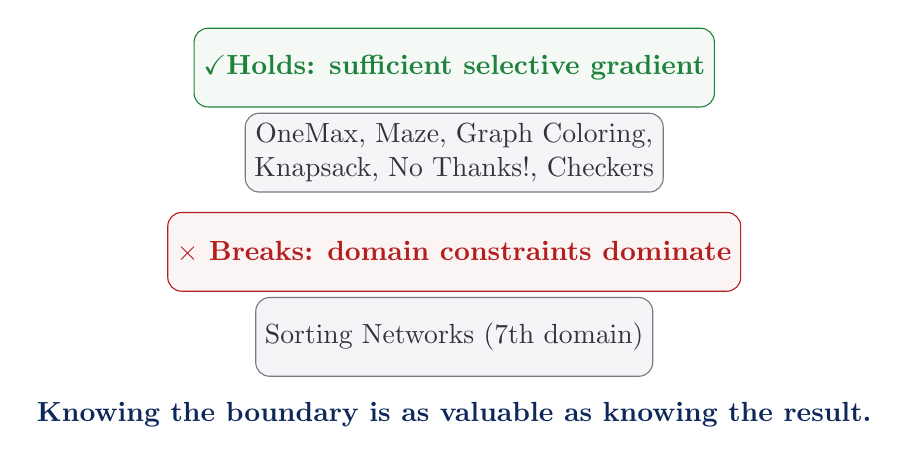
\begin{tikzpicture}[scale=0.9,
  box/.style={draw=midgray,fill=lightgray,rounded corners=5pt,
              minimum width=5cm,minimum height=1cm,
              font=\normalsize,text=textgray,align=center},
  cbox/.style={draw=greenok,fill=white!95!greenok,rounded corners=5pt,
               minimum width=5cm,minimum height=1cm,
               font=\normalsize\bfseries,text=greenok,align=center},
  rbox/.style={draw=redbad,fill=white!95!redbad,rounded corners=5pt,
               minimum width=5cm,minimum height=1cm,
               font=\normalsize\bfseries,text=redbad,align=center}
]
  \node[cbox] at (0, 1.5) {\checkmark Holds: sufficient selective gradient};
  \node[box]  at (0, 0.3) {OneMax, Maze, Graph Coloring,\\Knapsack, No Thanks!, Checkers};
  \node[rbox] at (0,-1.1) {$\times$ Breaks: domain constraints dominate};
  \node[box]  at (0,-2.3) {Sorting Networks (7th domain)};
  \node[font=\normalsize\bfseries,text=deepblue] at (0,-3.4)
    {Knowing the boundary is as valuable as knowing the result.};
\end{tikzpicture}
\end{center}
\end{frame}

% --- Slide 15: Four Strategy Compositions ---
\begin{frame}{Four Strategy Compositions}
\begin{columns}[T]
  \begin{column}{0.5\textwidth}
    \textbf{\color{accentblue}Generational}\\
    \small Same pipeline, repeated iteration.\\[0.4em]
    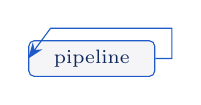
\begin{tikzpicture}[scale=0.7,
      b/.style={draw=accentblue,fill=lightgray,rounded corners=2pt,
                minimum width=1.6cm,minimum height=0.45cm,
                font=\scriptsize,text=deepblue}]
      \node[b] (p) at (0,0) {pipeline};
      \draw[-{Stealth[length=2mm]},color=accentblue]
        (p.east) -- ++(0.3,0) -- ++(0,0.55) -- ++(-2.2,0) -- (p.west);
    \end{tikzpicture}\\[0.8em]
    \textbf{\color{accentorange}Hourglass}\\
    \small Three explicit phases.\\[0.4em]
    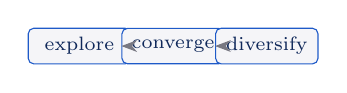
\begin{tikzpicture}[scale=0.7,
      b/.style={draw=accentblue,fill=lightgray,rounded corners=2pt,
                minimum width=1.3cm,minimum height=0.45cm,
                font=\scriptsize,text=deepblue},
      a/.style={-{Stealth[length=2mm]},color=midgray}]
      \node[b] (e1) at (0,0) {explore};
      \node[b] (cv) at (1.7,0) {converge};
      \node[b] (dv) at (3.4,0) {diversify};
      \draw[a] (e1) -- (cv); \draw[a] (cv) -- (dv);
    \end{tikzpicture}
  \end{column}
  \begin{column}{0.5\textwidth}
    \textbf{\color{greenok}Island}\\
    \small Parallel pipelines + ring migration.\\[0.4em]
    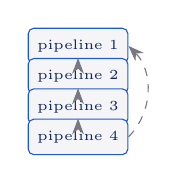
\begin{tikzpicture}[scale=0.7,
      b/.style={draw=accentblue,fill=lightgray,rounded corners=2pt,
                minimum width=1.1cm,minimum height=0.45cm,
                font=\tiny,text=deepblue},
      a/.style={-{Stealth[length=2mm]},color=midgray,dashed}]
      \foreach \i/\y in {1/1.1,2/0.55,3/0,4/-0.55} {
        \node[b] (p\i) at (0,\y) {pipeline \i};
      }
      \draw[a] (p1) -- (p2); \draw[a] (p2) -- (p3);
      \draw[a] (p3) -- (p4); \draw[a,bend right=45] (p4.east) to (p1.east);
    \end{tikzpicture}\\[0.8em]
    \textbf{\color{redbad}Adaptive}\\
    \small Plateau-triggered switch.\\[0.4em]
    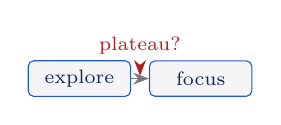
\begin{tikzpicture}[scale=0.7,
      b/.style={draw=accentblue,fill=lightgray,rounded corners=2pt,
                minimum width=1.3cm,minimum height=0.45cm,
                font=\scriptsize,text=deepblue},
      a/.style={-{Stealth[length=2mm]},color=midgray}]
      \node[b] (ex) at (0,0) {explore};
      \node[b] (fo) at (2.2,0) {focus};
      \node[font=\scriptsize,text=redbad] (sw) at (1.1,0.6) {plateau?};
      \draw[a] (ex) -- (fo);
      \draw[dashed,color=redbad,-{Stealth[length=2mm]}] (sw) -- (1.1,0.05);
    \end{tikzpicture}
  \end{column}
\end{columns}
\vspace{0.6em}
\begin{center}
\colorbox{lightgray}{\parbox{0.85\textwidth}{\centering
  \small\color{deepblue}Same base operators (evaluate, select, crossover, mutate) --- different recipes.
}}
\end{center}
\end{frame}

% --- Slide 16: Fingerprint Chart [AHA] ---
\begin{frame}{The Fingerprint Chart}
\begin{center}
  \includegraphics[width=0.88\textwidth]{fingerprints_panels.png}
\end{center}
\vspace{0.2em}
\begin{center}
\small
\textcolor{accentblue}{\textbf{Flat:} monotone decline to 0.13}\quad
\textcolor{greenok}{\textbf{Hourglass:} crash ($-85\%$) then rebound to 0.37}\quad
\textcolor{accentorange}{\textbf{Island:} diversity thermostat}\quad
\textcolor{redbad}{\textbf{Adaptive:} irreversible collapse to 0.02}\\[0.3em]
\textbf{\color{deepblue}Same operators. $18\times$ spread in final diversity. Shape determined by composition, not landscape.}
\end{center}
\end{frame}

% --- Slide 17: Fingerprints Stable Across Domains ---
\begin{frame}{Fingerprints Are Stable Across Domains}
\begin{columns}[T]
  \begin{column}{0.65\textwidth}
    \includegraphics[width=\textwidth]{multi_domain_panel.png}
  \end{column}
  \begin{column}{0.32\textwidth}
    \vspace{0.5em}
    \begin{itemize}\setlength\itemsep{0.6em}
      \item Hourglass crash: \textbf{same relative point} in every domain
      \item Island thermostat: \textbf{same relative level}
      \item Adaptive collapse: \textbf{equally irreversible} everywhere
    \end{itemize}
    \vspace{0.8em}
    \colorbox{lightgray}{\parbox{\textwidth}{
      \small\color{accentblue}
      Predict diversity trajectory from composition alone --- before running a single experiment.
    }}
  \end{column}
\end{columns}
\end{frame}

% --- Slide 18: Three Recommendations ---
\begin{frame}{Three Recommendations for Practitioners}
\begin{columns}[T]
  \begin{column}{0.55\textwidth}
    \includegraphics[width=\textwidth]{before_after_topology.png}
  \end{column}
  \begin{column}{0.42\textwidth}
    \vspace{0.3em}
    \begin{enumerate}\setlength\itemsep{0.7em}
      \item \textbf{Prefer ring/mesh over star}\\
        \small Star has $\beta_1 = 0$ (no cycles). Add a ring: $n-1$ cycles at zero extra edge cost.
      \item \textbf{Monitor $\lambda_2$, not diversity}\\
        \small Cheap (one eigenvalue). Predicts collapse \textbf{50--100 gen early}.
      \item \textbf{Close cycles, don't raise migration rate}\\
        \small Higher rate = more coupling, same topology. One edge changes both.
    \end{enumerate}
  \end{column}
\end{columns}
\end{frame}

% --- Slide 19: Summary ---
\begin{frame}{Summary}
\begin{columns}[T]
  \begin{column}{0.42\textwidth}
    \vspace{0.5em}
    \begin{center}
    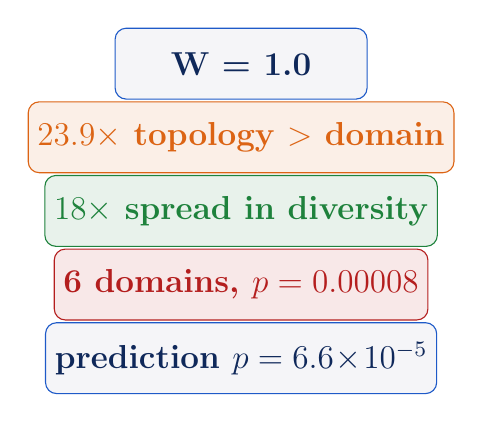
\begin{tikzpicture}[scale=0.85,
      stat/.style={draw=accentblue,fill=lightgray,rounded corners=4pt,
                   minimum width=3.2cm,minimum height=0.9cm,
                   font=\large\bfseries,text=deepblue,align=center}]
      \node[stat] at (0,2.8) {W = 1.0};
      \node[stat,fill=white!90!accentorange,draw=accentorange,text=accentorange] at (0,1.7) {$23.9\times$ topology $>$ domain};
      \node[stat,fill=white!90!greenok,draw=greenok,text=greenok] at (0,0.6) {$18\times$ spread in diversity};
      \node[stat,fill=white!90!redbad,draw=redbad,text=redbad] at (0,-0.5) {6 domains, $p=0.00008$};
      \node[stat] at (0,-1.6) {prediction $p = 6.6\!\times\!10^{-5}$};
    \end{tikzpicture}
    \end{center}
  \end{column}
  \begin{column}{0.55\textwidth}
    \vspace{0.5em}
    \begin{itemize}\setlength\itemsep{0.55em}
      \item \textbf{Composition determines diversity} --- empirically, across 6 domains
      \item \textbf{Universal topology ordering} explained by spectral graph theory
      \item \textbf{Novel prediction confirmed:} ring/star inversion at $n=7$
      \item \textbf{Diversity fingerprints} are properties of composition patterns, not operators
      \item \textbf{Categorical framework} (Kleisli arrows) makes structure visible and formally analyzable
    \end{itemize}
    \vspace{0.5em}
    \small\color{midgray}\textit{Future: larger populations, heterogeneous island strategies}
  \end{column}
\end{columns}
\end{frame}

% --- Slide 20: Thank You ---
{
\setbeamertemplate{footline}{}
\begin{frame}[plain]
\begin{center}
  \vspace{2em}
  {\Huge\bfseries\color{deepblue} Thank You}\\[1.2em]
  {\large\color{textgray} Composition Determines Diversity}\\
  {\normalsize\color{midgray} Categorical Fingerprints of Genetic Algorithms}\\[1.2em]
  \color{accentblue}{\rule{0.5\textwidth}{1.2pt}}\\[1.2em]
  {\normalsize\color{textgray}
    Robin Langer \quad Claudius Turing \quad Lyra Vega\\[0.4em]
    \texttt{langer.robin@gmail.com}
  }\\[1em]
  {\small\color{midgray}
    Code \& paper: \texttt{github.com/lyra-claude/categorical-evolution}\\[0.3em]
    GECCO 2026 \textbullet{} San Jos\'e, Costa Rica
  }
\end{center}
\end{frame}
}

\end{document}
